% !TeX program = xelatex
% گزارش پروژه نهایی درس مبانی اینترنت اشیا
% پیشنهاد: دو بار با XeLaTeX کامپایل شود.

\documentclass[11pt,a4paper,oneside]{article}
\setlength{\emergencystretch}{5em}

\usepackage[a4paper,margin=0.82in]{geometry}
\usepackage{xcolor}
\usepackage{graphicx}
\usepackage{amsmath,amssymb,mathtools}
\usepackage{enumitem}
\usepackage{etoolbox}
\usepackage{xparse}
\usepackage[most]{tcolorbox}
\usepackage{hyperref}
\usepackage{tabularx}
\usepackage{booktabs}
\usepackage{array}
\usepackage{float}
\usepackage{xepersian}

% همان الگوی کلی نمونه: XeLaTeX + xepersian، متن فارسی و قطعات لاتین صریح.
\IfFileExists{Vazirmatn.ttf}{%
  \settextfont[Path=./,Scale=1.02,BoldFont={Vazirmatn-Bold.ttf}]{Vazirmatn.ttf}%
  \setlatintextfont[Path=./,Scale=.94,BoldFont={Vazirmatn-Bold.ttf}]{Vazirmatn.ttf}%
}{%
  \settextfont[Scale=1.02]{DejaVu Sans}%
  \setlatintextfont[Scale=.94]{DejaVu Sans}%
}

\definecolor{Ink}{HTML}{172B3A}
\definecolor{Accent}{HTML}{087F8C}
\definecolor{Pale}{HTML}{EDF7F8}
\definecolor{Muted}{HTML}{536773}
\definecolor{Warn}{HTML}{8A4B08}

\hypersetup{
  unicode=true,
  colorlinks=true,
  linkcolor=Ink,
  citecolor=Ink,
  urlcolor=blue,
  pdftitle={گزارش پروژه سامانه هوشمند اینترنت اشیا مبتنی بر ESP32-CAM، Arduino، Telegram و مدل زبانی},
  pdfauthor={سپهر رجبی و امیرحسین جعفری}
}

\graphicspath{{figures/}}

\newcommand{\StudentOneName}{سپهر رجبی}
\newcommand{\StudentOneID}{۴۰۱۳۶۲۳۰۰۸}
\newcommand{\StudentTwoName}{امیرحسین جعفری}
\newcommand{\StudentTwoID}{۴۰۱۳۶۱۳۰۱۵}
\newcommand{\InstructorName}{دکتر علی بهلولی}
\newcommand{\CourseName}{مبانی اینترنت اشیا}
\newcommand{\SemesterName}{بهار ۱۴۰۳}
\newcommand{\Eng}[1]{\lr{#1}}
\newcommand{\term}[1]{\textbf{#1}}
\newcommand{\code}[1]{\lr{\texttt{#1}}}
\newcommand{\pathcode}[1]{\lr{\ttfamily #1}}

\setlength{\parindent}{0pt}
\setlength{\parskip}{0.43em}
\linespread{1.08}
\setlist[itemize]{topsep=.25em,itemsep=.18em,rightmargin=1.15em,leftmargin=0pt,label=\textcolor{Accent}{\tiny$\blacksquare$}}
\setlist[enumerate]{topsep=.25em,itemsep=.22em,rightmargin=1.35em,leftmargin=0pt}

\makeatletter
\renewcommand\section{\@startsection{section}{1}{\z@}%
  {1.0em}{0.35em}{\color{Accent}\bfseries\fontsize{14.3}{17}\selectfont}}
\renewcommand\subsection{\@startsection{subsection}{2}{\z@}%
  {.75em}{.22em}{\color{Ink}\bfseries\fontsize{12.4}{15}\selectfont}}
\renewcommand\subsubsection{\@startsection{subsubsection}{3}{\z@}%
  {.55em}{.18em}{\color{Muted}\bfseries\fontsize{11.4}{14}\selectfont}}
\renewcommand{\@biblabel}[1]{\lr{[#1]}}
\makeatother

\newtcolorbox{summarybox}{
  enhanced,colback=Pale,colframe=Accent,boxrule=.7pt,arc=2mm,
  left=7pt,right=7pt,top=6pt,bottom=6pt,
  width=.97\textwidth,center,before skip=6pt,after skip=7pt
}
\newtcolorbox{notebox}{
  enhanced,colback=gray!3,colframe=gray!55,boxrule=.5pt,arc=1.8mm,
  left=7pt,right=7pt,top=5pt,bottom=5pt,
  width=.97\textwidth,center,before skip=5pt,after skip=6pt
}
\newtcolorbox{warningbox}{
  enhanced,colback=orange!4,colframe=Warn,boxrule=.65pt,arc=1.8mm,
  left=7pt,right=7pt,top=5pt,bottom=5pt,
  width=.97\textwidth,center,before skip=5pt,after skip=6pt
}

\newcolumntype{R}[1]{>{\raggedleft\arraybackslash}p{#1}}
\newcolumntype{C}[1]{>{\centering\arraybackslash}p{#1}}
\pagestyle{plain}

\begin{document}

% -----------------------------------------------------------------------------
% جلد
% -----------------------------------------------------------------------------
\begingroup
\thispagestyle{empty}
\centering
\vspace*{1.1cm}
\begin{tcolorbox}[width=4.4cm,height=2.0cm,colback=Pale,colframe=Accent,arc=4mm,boxrule=1pt,valign=center]
\centering{\Huge\bfseries\Eng{IoT}}\\[-1mm]
{\small\color{Muted}\Eng{ESP32-CAM + Arduino}}
\end{tcolorbox}
\vspace{1.1cm}

{\Large\textbf{گزارش پروژهٔ درس \CourseName}}\par
\vspace{0.65cm}
{\normalsize\textbf{عنوان پروژه}}\par
\vspace{0.2cm}
{\LARGE\textbf{طراحی و پیاده‌سازی سامانهٔ هوشمند اینترنت اشیا برای کنترل چندرابطه‌ای تجهیزات، دریافت تصویر و فرمان صوتی/متنی}}\par
\vspace{0.3cm}
{\large\Eng{Intelligent Multi-Interface IoT Control with ESP32-CAM, Arduino, Telegram, Voice, and LLM Commands}}\par

\vspace{1.15cm}
\begin{tcolorbox}[width=.79\textwidth,colback=white,colframe=gray!45,arc=2mm,boxrule=.55pt,left=8pt,right=8pt,top=8pt,bottom=8pt]
\centering
\textbf{استاد درس:} \InstructorName\\[6pt]
\textbf{اعضای گروه:}\\[4pt]
\StudentOneName{} \quad -- \quad \StudentOneID\\[3pt]
\StudentTwoName{} \quad -- \quad \StudentTwoID
\end{tcolorbox}

\vspace{0.75cm}
{\large \SemesterName}\par
\vfill
{\small\color{Muted}نسخهٔ گزارش بر پایهٔ کدهای پروژه و اسکریپت تشخیص چهرهٔ ارائه‌شده تهیه شده است.}
\clearpage
\endgroup

\setcounter{page}{1}

% -----------------------------------------------------------------------------
\section*{چکیده}
\addcontentsline{toc}{section}{چکیده}
پروژهٔ حاضر یک سامانهٔ اینترنت اشیای چندرابطه‌ای را پیاده‌سازی می‌کند که در آن یک \Eng{ESP32-CAM}، یک برد \Eng{Arduino} و یک رایانهٔ میزبان به‌صورت هم‌زمان در چرخهٔ دریافت فرمان، تفسیر فرمان، کنترل عملگر و دریافت تصویر مشارکت دارند. \Eng{ESP32-CAM} در نقش دروازهٔ محلی، نقطهٔ دسترسی \Eng{Wi-Fi} و وب‌سرور را ایجاد می‌کند، امکان ورود کاربر، ارسال فرمان متنی و درخواست تصویربرداری را فراهم می‌سازد و دو خروجی نوری را کنترل می‌کند. \Eng{Arduino} نیز دو \Eng{LED} و یک بازر را از طریق پیوند سریال کنترل می‌کند. در لایهٔ رایانه، برنامهٔ پایتون به‌عنوان هماهنگ‌کننده، ارتباط سریال با هر دو برد، ربات تلگرام، دریافت پیام صوتی، تبدیل گفتار به متن و نگاشت فرمان طبیعی به الفبای کنترلی محدود \Eng{A--L} را مدیریت می‌کند. علاوه بر این، تصویر گرفته‌شده با دوربین در یک قاب باینری مشخص از طریق \Eng{UART} به رایانه انتقال می‌یابد.

در کد جداگانهٔ ارائه‌شده، از کتابخانهٔ \Eng{DeepFace} برای تطبیق یک تصویر پرس‌وجو با چند تصویر مرجع استفاده شده است؛ این ماژول در نسخهٔ اولیه به خط لولهٔ اصلی متصل نیست و بنابراین در این گزارش به‌عنوان قابلیت مکمل تحلیل می‌شود. تحلیل مهندسی پروژه نشان می‌دهد که ایدهٔ مرکزی، یعنی جداکردن «رابط کاربر و استدلال نرم‌افزاری» از «کنترل قطعی سخت‌افزار»، طراحی مناسبی برای یک نمونهٔ آموزشی است. بااین‌حال، نسخهٔ اولیه دارای محدودیت‌هایی از جمله ذخیرهٔ مستقیم کلیدهای سرویس در کد، دو منطق موازی برای دریافت تصویر، عدم تطابق رفتار اسکریپت درخواست تصویر با پروتکل واقعی، و ساده‌بودن احراز هویت وب است. نسخهٔ آمادهٔ گیت‌هاب همراه این گزارش این موارد را تا حد ممکن بدون تغییر ماهیت پروژه اصلاح و مستندسازی می‌کند.

\textbf{واژگان کلیدی:} اینترنت اشیا، \Eng{ESP32-CAM}، \Eng{Arduino}، \Eng{UART}، تلگرام، فرمان صوتی، مدل زبانی، \Eng{DeepFace}، کنترل عملگر، انتقال تصویر.

\begin{summarybox}
\textbf{خلاصهٔ معماری:} ورودی کاربر از وب محلی یا تلگرام دریافت می‌شود؛ پیام صوتی در صورت نیاز به متن تبدیل می‌شود؛ یک مدل زبانی فقط نقش نگاشت‌کنندهٔ زبان طبیعی به حروف کنترلی را دارد؛ سپس برنامهٔ پایتون حروف معتبر را به \Eng{ESP32-CAM} یا \Eng{Arduino} می‌فرستد. مسیر تصویر مستقل است: درخواست \code{/capture} در وب، تصویربرداری را فعال می‌کند و \Eng{JPEG} با قالب \code{START\_IMG + length + payload + END\_IMG} روی سریال به رایانه بازمی‌گردد.
\end{summarybox}

\tableofcontents
\clearpage

% -----------------------------------------------------------------------------
\section{مقدمه و تعریف مسئله}
هدف پروژه، ساخت یک نمونهٔ عملی از یک سامانهٔ اینترنت اشیا است که صرفاً یک «کلید روشن/خاموش تحت شبکه» نباشد، بلکه چند نوع رابط ورودی و چند گرهٔ سخت‌افزاری را زیر یک منطق هماهنگ‌کننده یکپارچه کند. در این معماری، کاربر می‌تواند از طریق مرورگر متصل به شبکهٔ محلی \Eng{ESP32}، پیام تلگرام یا پیام صوتی فرمان بدهد؛ رایانه فرمان را پردازش و به یک پروتکل بسیار کوچک و قطعی تبدیل می‌کند؛ سپس عملگر متناظر روی یکی از دو برد فعال می‌شود. هم‌زمان، دوربین \Eng{ESP32-CAM} قابلیت تصویربرداری و انتقال فایل باینری به میزبان را نیز فراهم می‌کند.

از دید اینترنت اشیا، پروژه چهار مؤلفهٔ اصلی را پوشش می‌دهد: \term{حسگری} از طریق دوربین، \term{عملگری} با \Eng{LED} و بازر، \term{ارتباط} با \Eng{Wi-Fi/HTTP} و \Eng{UART}، و \term{هوشمندی/هماهنگ‌سازی} در لایهٔ نرم‌افزار رایانه. این جداسازی با برداشت کلاسیک از سامانه‌های \Eng{IoT} به‌عنوان شبکه‌ای از اشیای فیزیکی دارای قابلیت حس، ارتباط و کنش سازگار است \cite{atzori2010}.

\subsection{مبنای تحلیل گزارش}
این گزارش از روی فایل‌های پیاده‌سازی ارائه‌شده بازسازی شده است: برنامهٔ اصلی پایتون، برنامهٔ کمکی درخواست تصویر، کد \Eng{Arduino}، کد \Eng{ESP32-CAM} و اسکریپت مستقل تشخیص چهره. بنابراین هرجا میان «رفتار مورد انتظار» و «رفتار واقعی کد» اختلاف وجود داشته، رفتار واقعی کد مبنا قرار گرفته و اختلاف به‌صورت شفاف در بخش محدودیت‌ها توضیح داده شده است.

% -----------------------------------------------------------------------------
\section{اهداف عملکردی و سناریوهای کاربری}
می‌توان نیازمندی‌های پروژه را به شش سناریوی اصلی تقسیم کرد:
\begin{enumerate}
\item \term{ورود از وب محلی:} کاربر به نقطهٔ دسترسی \Eng{ESP32} متصل شده، نام کاربری و رمز را وارد می‌کند و در صورت موفقیت به صفحهٔ پیام هدایت می‌شود.
\item \term{فرمان متنی از وب:} متن طبیعی کاربر از صفحهٔ وب روی سریال چاپ می‌شود، رایانه آن را دریافت و به یک یا چند حرف کنترلی تبدیل می‌کند.
\item \term{فرمان متنی تلگرام:} در صورتی که هنگام ورود گزینهٔ تلگرام فعال شده باشد، ربات تلگرام پیام کاربر را دریافت و از همان خط لولهٔ تفسیر فرمان عبور می‌دهد.
\item \term{فرمان صوتی تلگرام:} پیام صوتی دانلود، از \Eng{OGG} به \Eng{WAV} تبدیل و با موتور تشخیص گفتار به متن تبدیل می‌شود؛ خروجی متنی سپس مانند سایر فرمان‌ها پردازش می‌شود.
\item \term{بازخورد ورود ناموفق:} در نسخهٔ پروژه، پیام خطای ورود از \Eng{ESP32} به رایانه می‌رسد و رایانه با فرمان‌های \code{K} و \code{L} بازر آردوینو را برای مدت کوتاه فعال می‌کند.
\item \term{تصویربرداری:} کاربر مسیر \code{/capture} را فراخوانی می‌کند؛ دوربین فریم \Eng{JPEG} می‌گیرد و تصویر به‌صورت باینری روی \Eng{UART} به میزبان انتقال داده می‌شود.
\end{enumerate}

% -----------------------------------------------------------------------------
\section{معماری کلان سامانه}
شکل \ref{fig:architecture} توپولوژی منطقی پروژه را نشان می‌دهد. نکتهٔ کلیدی این است که مدل زبانی مستقیماً به پایه‌های سخت‌افزار دسترسی ندارد. خروجی مدل ابتدا توسط برنامهٔ میزبان به مجموعهٔ محدود حروف معتبر تقلیل داده شده و سپس بر اساس مقصد به پورت سریال مناسب فرستاده می‌شود. این جداسازی، فضای خروجی را از زبان آزاد به یک پروتکل کوچک تبدیل می‌کند و امکان ممیزی رفتار را افزایش می‌دهد.

\begin{figure}[H]
\centering
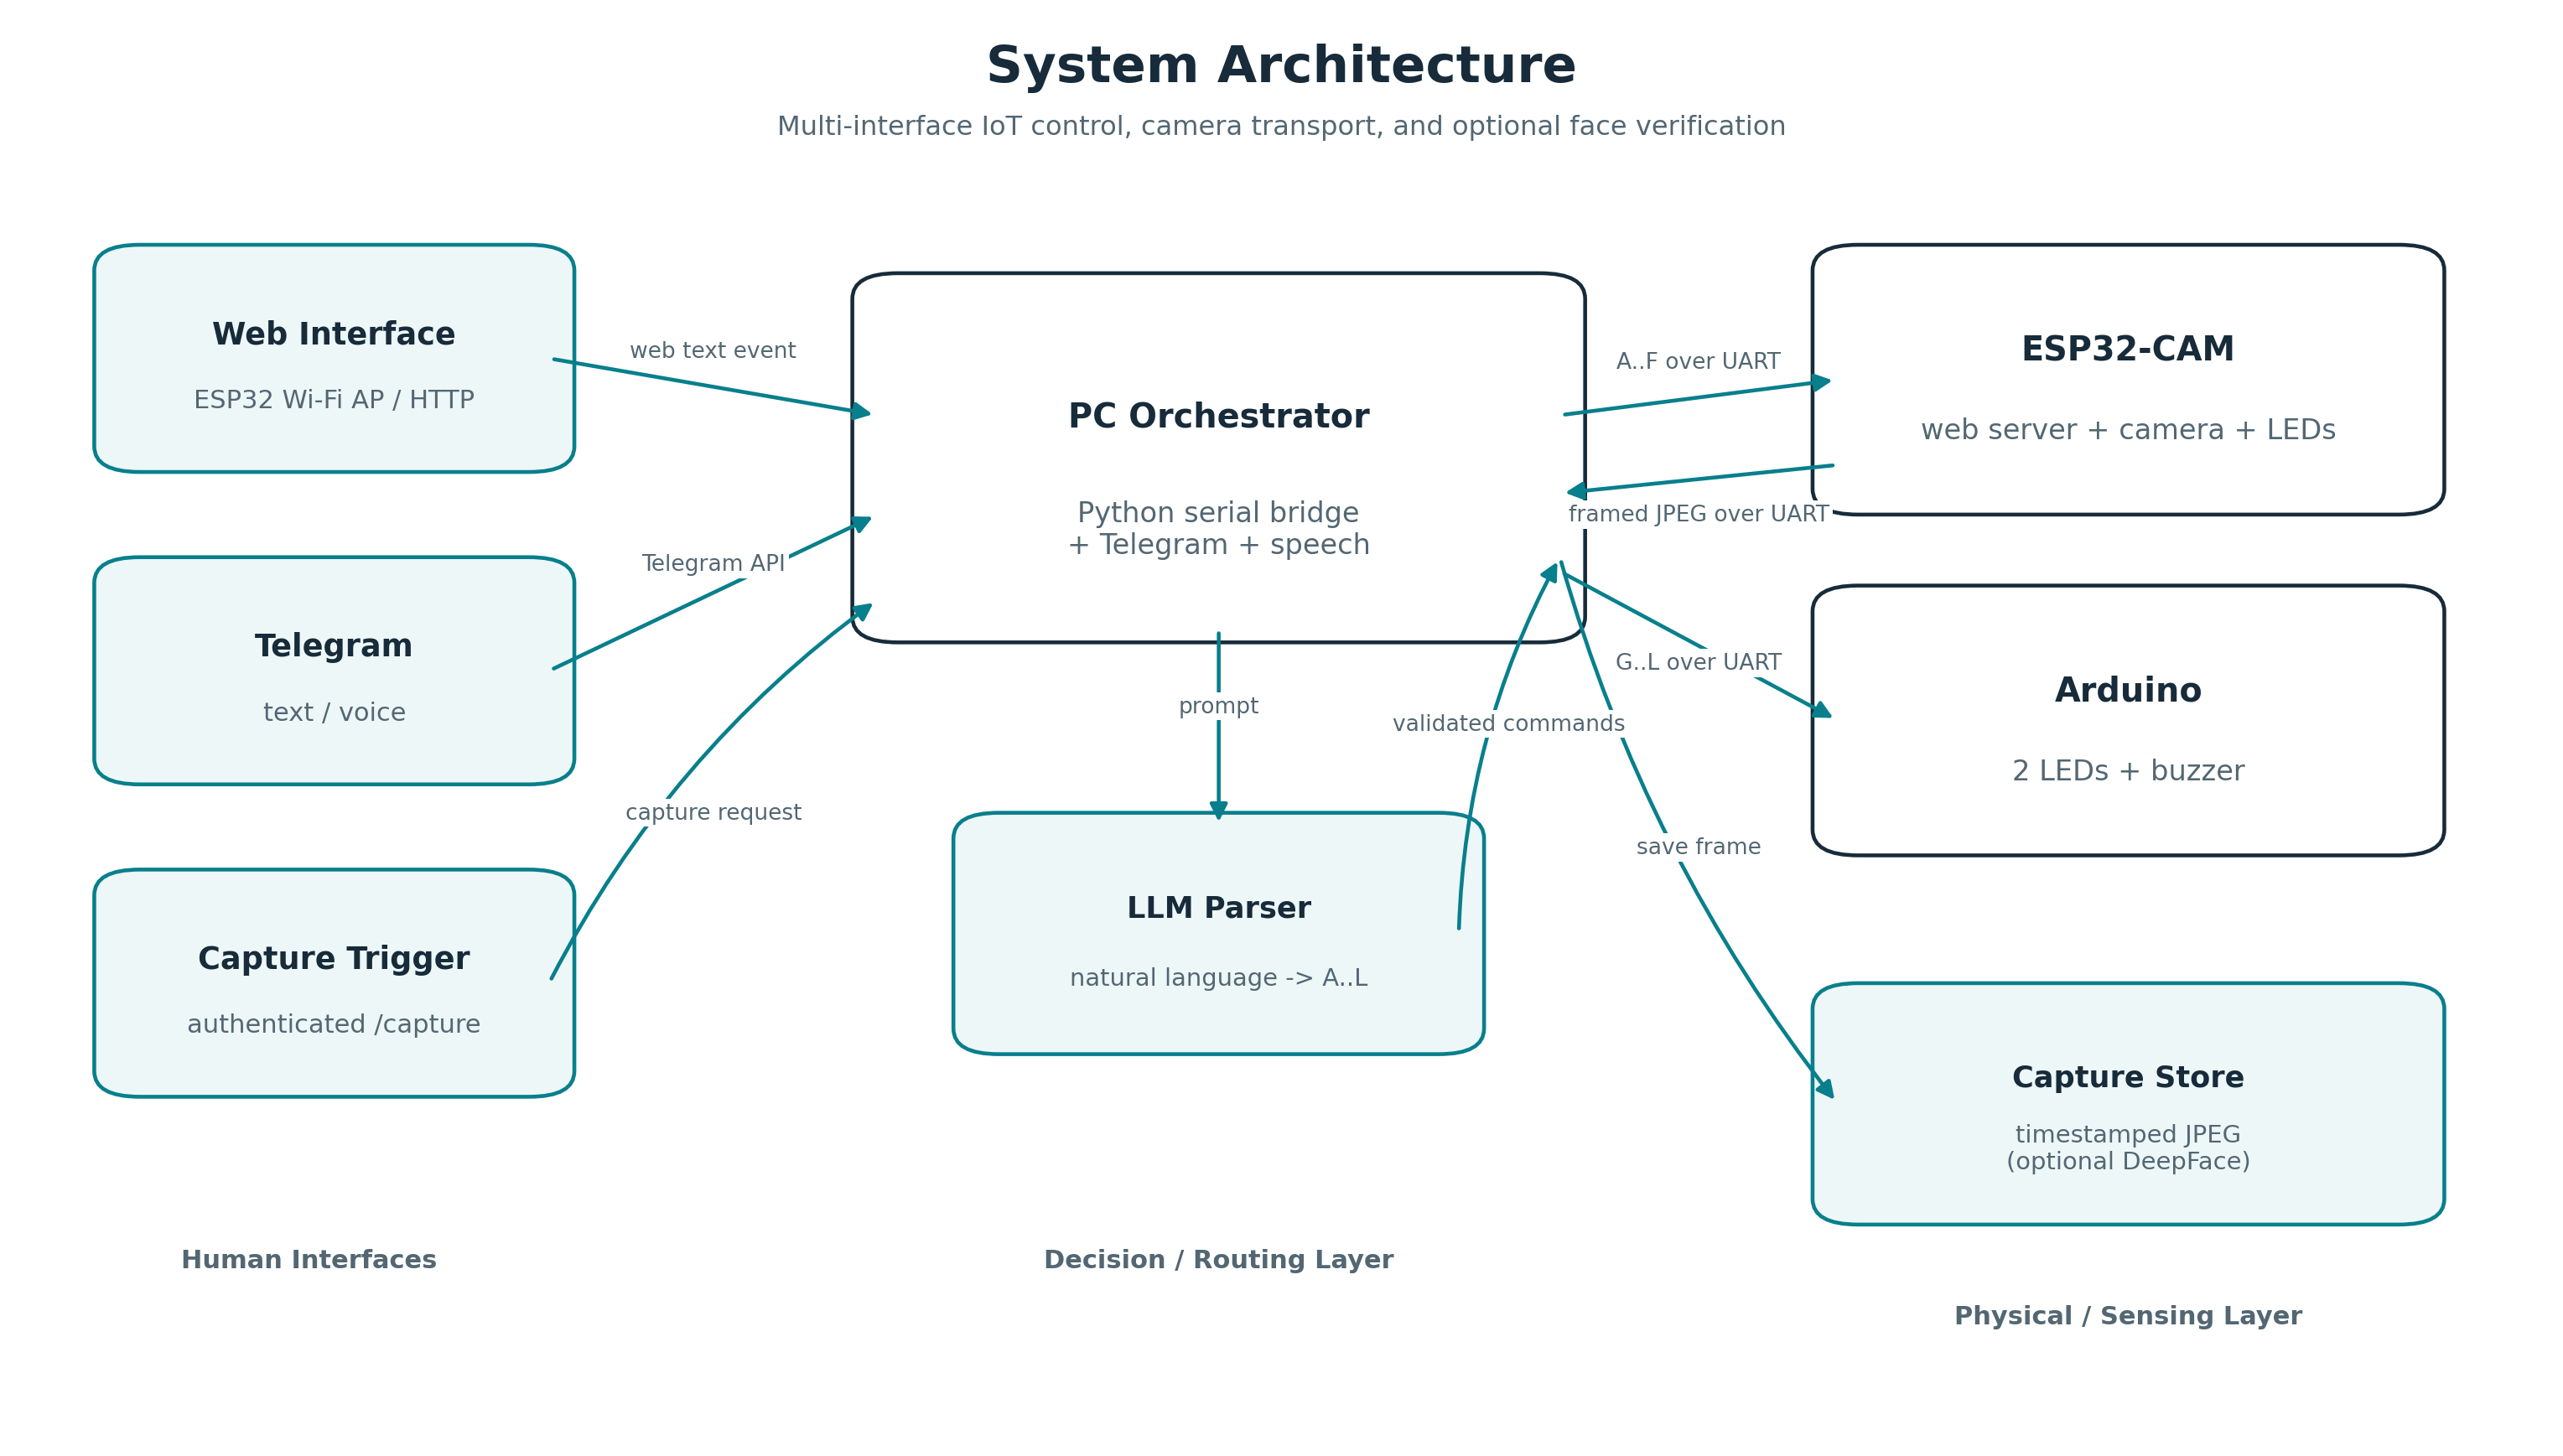
\includegraphics[width=.97\textwidth]{architecture.png}
\caption{معماری سطح‌بالای سامانه و مسیرهای اصلی داده و فرمان}
\label{fig:architecture}
\end{figure}

\subsection{لایهٔ رابط انسانی}
رابط وب در خود \Eng{ESP32-CAM} میزبانی می‌شود و برای اجرای سناریو به سرویس‌دهندهٔ وب جداگانه نیاز ندارد. تلگرام و پیام صوتی در سمت رایانه مدیریت می‌شوند. از نظر معماری، این دو مسیر در نقطهٔ «متن فرمان» به یکدیگر می‌رسند؛ یعنی پس از تبدیل صوت به متن، تفاوتی میان فرمان وب، تلگرام یا گفتار وجود ندارد.

\subsection{لایهٔ هماهنگ‌کننده}
برنامهٔ پایتون واسط میان همهٔ سرویس‌هاست: دو پورت سریال را باز می‌کند، پیام‌های وضعیت \Eng{ESP32} را می‌خواند، ربات تلگرام را در یک رشتهٔ جداگانه اجرا می‌کند، صوت را تبدیل و تشخیص می‌دهد، مدل زبانی را فراخوانی می‌کند و در نهایت فرمان را مسیریابی می‌کند. از این رو رایانه عملاً نقش \Eng{edge gateway/orchestrator} را دارد.

\subsection{لایهٔ فیزیکی}
\Eng{ESP32-CAM} هم گرهٔ حسگر و هم گرهٔ عملگر است؛ \Eng{Arduino} گرهٔ عملگر دوم است. در طراحی ارائه‌شده، هر دو برد از طریق اتصال سریال مستقل به رایانه وصل هستند و نرخ تبادل هر دو \Eng{115200 baud} است.

% -----------------------------------------------------------------------------
\section{سخت‌افزار و نگاشت پایه‌ها}
\begin{table}[H]
\centering
\caption{خلاصهٔ اجزای سخت‌افزاری قابل استخراج از کد}
\begin{tabularx}{.96\textwidth}{R{3.2cm} R{3.1cm} X}
\toprule
\textbf{گره} & \textbf{پایه/واسط} & \textbf{کارکرد}\\
\midrule
\Eng{ESP32-CAM} & \Eng{GPIO 4} & خروجی نوری اول؛ در بسیاری از بردهای \Eng{AI Thinker} این پایه با فلش روی برد نیز مرتبط است.\\
\Eng{ESP32-CAM} & \Eng{GPIO 33} & خروجی نوری دوم؛ منطق موجود در پروژه برای روشن/خاموش آن معکوس است و عملاً سیم‌بندی \Eng{active-low} را نشان می‌دهد.\\
\Eng{ESP32-CAM} & رابط دوربین & پیکربندی استاندارد پین‌های دوربین نوع \Eng{AI Thinker} و خروجی \Eng{JPEG}.\\
\Eng{Arduino} & \Eng{D2} & \Eng{LED 1}.\\
\Eng{Arduino} & \Eng{D4} & \Eng{LED 2}.\\
\Eng{Arduino} & \Eng{D3} & بازر.\\
رایانه & دو پورت سریال & یک اتصال مستقل برای \Eng{ESP32-CAM} و یک اتصال برای \Eng{Arduino}.\\
\bottomrule
\end{tabularx}
\end{table}

در کد اولیه، فرمان‌های \code{E} و \code{F} برای \Eng{LED 3} تعریف شده‌اند اما پایهٔ مربوطه به دلیل تعارض/محدودیت سخت‌افزاری غیرفعال شده است. بنابراین این دو فرمان در پیاده‌سازی واقعی اثری ندارند. نسخهٔ آمادهٔ مخزن، آن‌ها را به‌صراحت به‌عنوان \term{رزرو شده} علامت‌گذاری می‌کند تا قرارداد نرم‌افزار با وضعیت سخت‌افزار اشتباه نشود.

% -----------------------------------------------------------------------------
\section{نرم‌افزار ESP32-CAM و رابط وب}
کد \Eng{ESP32-CAM} سه وظیفهٔ عمده دارد: راه‌اندازی دوربین، ساخت شبکهٔ \Eng{Wi-Fi} در حالت \Eng{SoftAP}، و ارائهٔ وب‌سرور محلی. در نسخهٔ اولیه، \Eng{SSID} برابر \code{ESP32} بوده و کاربر پس از اتصال معمولاً از نشانی محلی پیش‌فرض \code{192.168.4.1} استفاده می‌کند.

\subsection{راه‌اندازی دوربین}
دوربین با قالب \Eng{PIXFORMAT\_JPEG}، وضوح \Eng{QVGA} معادل $320\times240$ و یک \Eng{frame buffer} تنظیم شده است. انتخاب وضوح پایین در این پروژه منطقی است، زیرا مسیر انتقال تصویر، \Eng{UART} با نرخ ۱۱۵۲۰۰ باود است و نه یک مسیر پرسرعت شبکه. در کتابخانهٔ رسمی \Eng{esp32-camera} نیز دریافت فریم بر پایهٔ \code{esp\_camera\_fb\_get()} انجام می‌شود \cite{esp32camera}.

\subsection{مسیرهای وب}
سه مسیر اصلی تعریف شده است:
\begin{itemize}
\item \code{/}: صفحهٔ ورود و دریافت وضعیت فعال‌سازی ربات تلگرام؛
\item \code{/message}: صفحهٔ ارسال فرمان طبیعی؛ متن از طریق \code{Serial.println} به رایانه ارسال می‌شود؛
\item \code{/capture}: ثبت تصویر و ارسال آن روی سریال.
\end{itemize}

پس از ورود موفق، \Eng{ESP32} یکی از دو پیام متنی «ورود موفق با تلگرام فعال» یا «ورود موفق» را روی سریال می‌فرستد. برنامهٔ پایتون دقیقاً از همین رشته برای تصمیم دربارهٔ راه‌اندازی ربات استفاده می‌کند. این طراحی ساده است و برای آزمایشگاه خوانایی خوبی دارد، اما وابستگی شدید به رشته‌های متنی دقیق ایجاد می‌کند؛ در نسخهٔ صنعتی بهتر است پیام‌های کنترلی ساخت‌یافته باشند.

% -----------------------------------------------------------------------------
\section{الفبای فرمان و مسیریابی قطعی}
برای جداکردن زبان طبیعی از فرمان سخت‌افزاری، پروژه یک الفبای کوچک از \Eng{A} تا \Eng{L} تعریف کرده است. جدول \ref{tab:commands} نگاشت واقعی این حروف را نشان می‌دهد.

\begin{table}[H]
\centering
\caption{قرارداد فرمان میان نرم‌افزار میزبان و میکروکنترلرها}
\label{tab:commands}
\begin{tabular}{C{2.0cm} C{3.0cm} R{6.6cm}}
\toprule
\textbf{فرمان} & \textbf{مقصد} & \textbf{عمل}\\
\midrule
\Eng{A} & \Eng{ESP32} & روشن‌کردن خروجی نوری ۱\\
\Eng{B} & \Eng{ESP32} & خاموش‌کردن خروجی نوری ۱\\
\Eng{C} & \Eng{ESP32} & روشن‌کردن خروجی نوری ۲، با منطق \Eng{active-low}\\
\Eng{D} & \Eng{ESP32} & خاموش‌کردن خروجی نوری ۲\\
\Eng{E/F} & \Eng{ESP32} & رزرو؛ خروجی سوم در سخت‌افزار ارائه‌شده متصل نیست\\
\Eng{G/H} & \Eng{Arduino} & روشن/خاموش‌کردن \Eng{LED 1}\\
\Eng{I/J} & \Eng{Arduino} & روشن/خاموش‌کردن \Eng{LED 2}\\
\Eng{K/L} & \Eng{Arduino} & روشن/خاموش‌کردن بازر\\
\bottomrule
\end{tabular}
\end{table}

اگر $x$ متن طبیعی ورودی و $f(x)$ خروجی مدل زبانی باشد، نسخهٔ امن‌تر منطق پروژه را می‌توان به‌صورت زیر نوشت:
\[
V = \{A,B,C,D,E,F,G,H,I,J,K,L\},\qquad
\hat{C}=\{c\in f(x)\mid c\in V\}.
\]
سپس تابع مسیریابی $g$ تنها بر اساس عضویت در دو زیرمجموعه عمل می‌کند:
\[
g(c)=
\begin{cases}
\mathrm{ESP32}, & c\in\{A,\dots,F\},\\
\mathrm{Arduino}, & c\in\{G,\dots,L\}.
\end{cases}
\]
این طراحی از نظر مهندسی مهم است: مدل زبانی «درایور سخت‌افزار» نیست؛ فقط مفسر ورودی طبیعی است و خروجی آن باید قبل از اعمال روی سخت‌افزار اعتبارسنجی شود.

\begin{figure}[H]
\centering
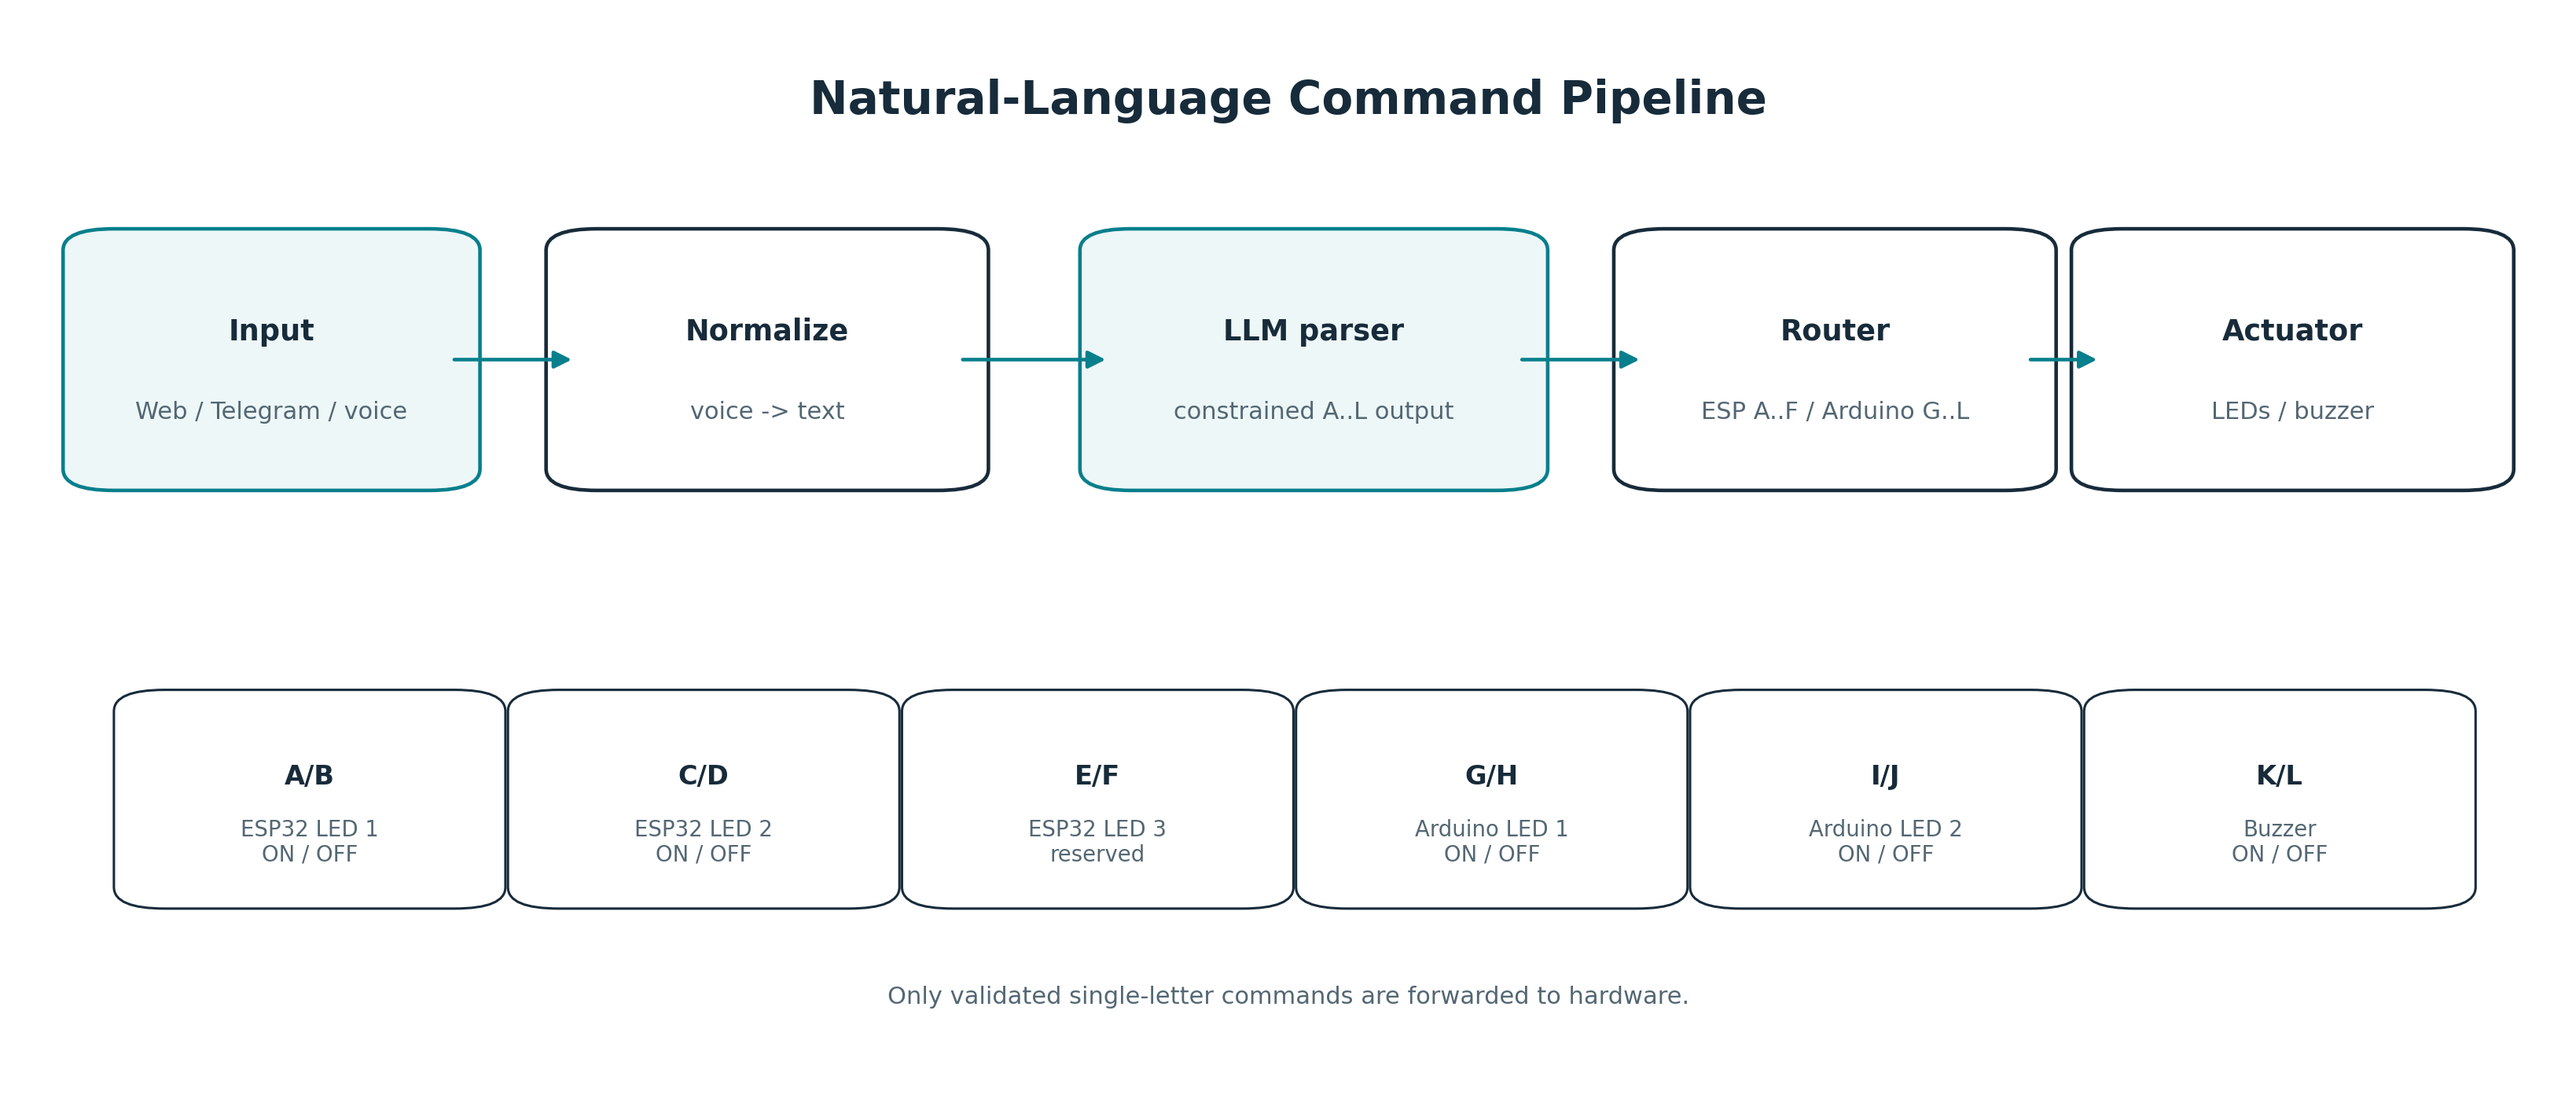
\includegraphics[width=.97\textwidth]{command_flow.png}
\caption{خط لولهٔ تبدیل فرمان طبیعی به پروتکل محدود و سپس مسیریابی به گرهٔ مناسب}
\end{figure}

% -----------------------------------------------------------------------------
\section{برنامهٔ پایتون به‌عنوان هماهنگ‌کنندهٔ مرکزی}
نسخهٔ اولیهٔ \code{IoT.py} مجموعهٔ بزرگی از مسئولیت‌ها را در یک فایل قرار داده است. با وجود تراکم، جریان اصلی آن را می‌توان به چهار زیرسامانه تفکیک کرد.

\subsection{مدیریت پورت‌های سریال}
دو پورت مستقل با نرخ یکسان باز می‌شوند. برای \Eng{ESP32}، سیگنال‌های \Eng{DTR/RTS} غیرفعال شده‌اند تا احتمال ریست ناخواستهٔ برد هنگام بازکردن پورت کاهش یابد. برنامه ابتدا منتظر پیام \code{CONFIG\_COMPLETE} می‌ماند و سپس وضعیت ورود را دنبال می‌کند.

\subsection{تفسیر زبان طبیعی با مدل زبانی}
در پرامپت سیستمی، معنای هر حرف \Eng{A--L} به مدل داده می‌شود و از مدل خواسته می‌شود صرفاً حروف معتبر، جداشده با فاصله، برگرداند. این الگو برای پروژهٔ آموزشی مناسب است، زیرا به‌جای تولید کد یا فراخوانی تابع آزاد، یک خروجی کوچک و قابل کنترل تولید می‌شود. نسخهٔ آمادهٔ گیت‌هاب یک مرحلهٔ اعتبارسنجی صریح نیز اضافه کرده است تا هر توکن خارج از مجموعهٔ مجاز حذف شود. استفاده از رابط \Eng{ChatOpenAI} از بستهٔ \Eng{LangChain} در این نقش با الگوی رایج فراخوانی یک مدل سازگار با \Eng{OpenAI API} هم‌راستا است \cite{langchain}.

\subsection{مدیریت رخدادهای ورود}
سه حالت اصلی از سریال تشخیص داده می‌شود: آماده‌شدن پیکربندی، ورود موفق، و ورود ناموفق. در حالت ورود ناموفق، برنامه \code{K} و سپس \code{L} را برای آردوینو می‌فرستد و یک بوق کوتاه ایجاد می‌کند. این یک نمونهٔ مناسب از پیوند میان رخداد نرم‌افزاری در گرهٔ شبکه و بازخورد فیزیکی در گرهٔ دیگر است.

\subsection{هم‌زمانی}
ربات تلگرام فقط در صورت فعال‌شدن گزینهٔ مربوطه راه‌اندازی می‌شود و در یک رشتهٔ جداگانه اجرا می‌گردد تا حلقهٔ سریال متوقف نشود. این انتخاب از نظر معماری صحیح است، هرچند در نسخهٔ عمومی باید مراقب مدیریت \Eng{event loop} و سیگنال‌ها در رشتهٔ فرعی بود. نسخهٔ آمادهٔ مخزن این بخش را با حلقهٔ رویداد مستقل و غیرفعال‌کردن سیگنال‌های توقف در رشتهٔ ربات پایدارتر می‌کند.

% -----------------------------------------------------------------------------
\section{تلگرام و فرمان صوتی}
در پروژه از چارچوب \Eng{python-telegram-bot} برای دریافت پیام‌ها استفاده شده است؛ ساخت \Eng{Application} و افزودن \Eng{MessageHandler} با الگوی نسخه‌های جدید این کتابخانه سازگار است \cite{ptb}.

برای پیام صوتی، فرایند زیر اجرا می‌شود:
\begin{enumerate}
\item فایل صوتی تلگرام بر اساس شناسهٔ فایل دانلود می‌شود؛
\item فایل \Eng{OGG} با کتابخانهٔ \Eng{soundfile} به \Eng{WAV} تبدیل می‌شود؛
\item \Eng{SpeechRecognition} فایل \Eng{WAV} را به سرویس تشخیص گفتار می‌فرستد؛
\item متن حاصل به کاربر بازگردانده و سپس، در صورت فعال‌بودن کنترل تلگرام، به مدل زبانی داده می‌شود؛
\item فایل‌های موقت صوتی پاک می‌شوند.
\end{enumerate}

مزیت مهم این معماری آن است که مسیر صوت پس از مرحلهٔ رونویسی، هیچ منطق کنترلی ویژه‌ای ندارد و از همان مسیر متن استفاده می‌کند. در نتیجه نگهداری منطق فرمان فقط در یک نقطه انجام می‌شود.

% -----------------------------------------------------------------------------
\section{پروتکل تصویربرداری و انتقال JPEG روی UART}
در \Eng{ESP32-CAM}، مسیر \code{/capture} با \code{esp\_camera\_fb\_get()} یک فریم می‌گیرد و سپس به‌جای برگرداندن تصویر در پاسخ \Eng{HTTP}، آن را روی سریال می‌فرستد. قاب ارسالی شامل یک نشانگر آغاز، طول تصویر، خود بایت‌های \Eng{JPEG} و نشانگر پایان است.

\begin{figure}[H]
\centering
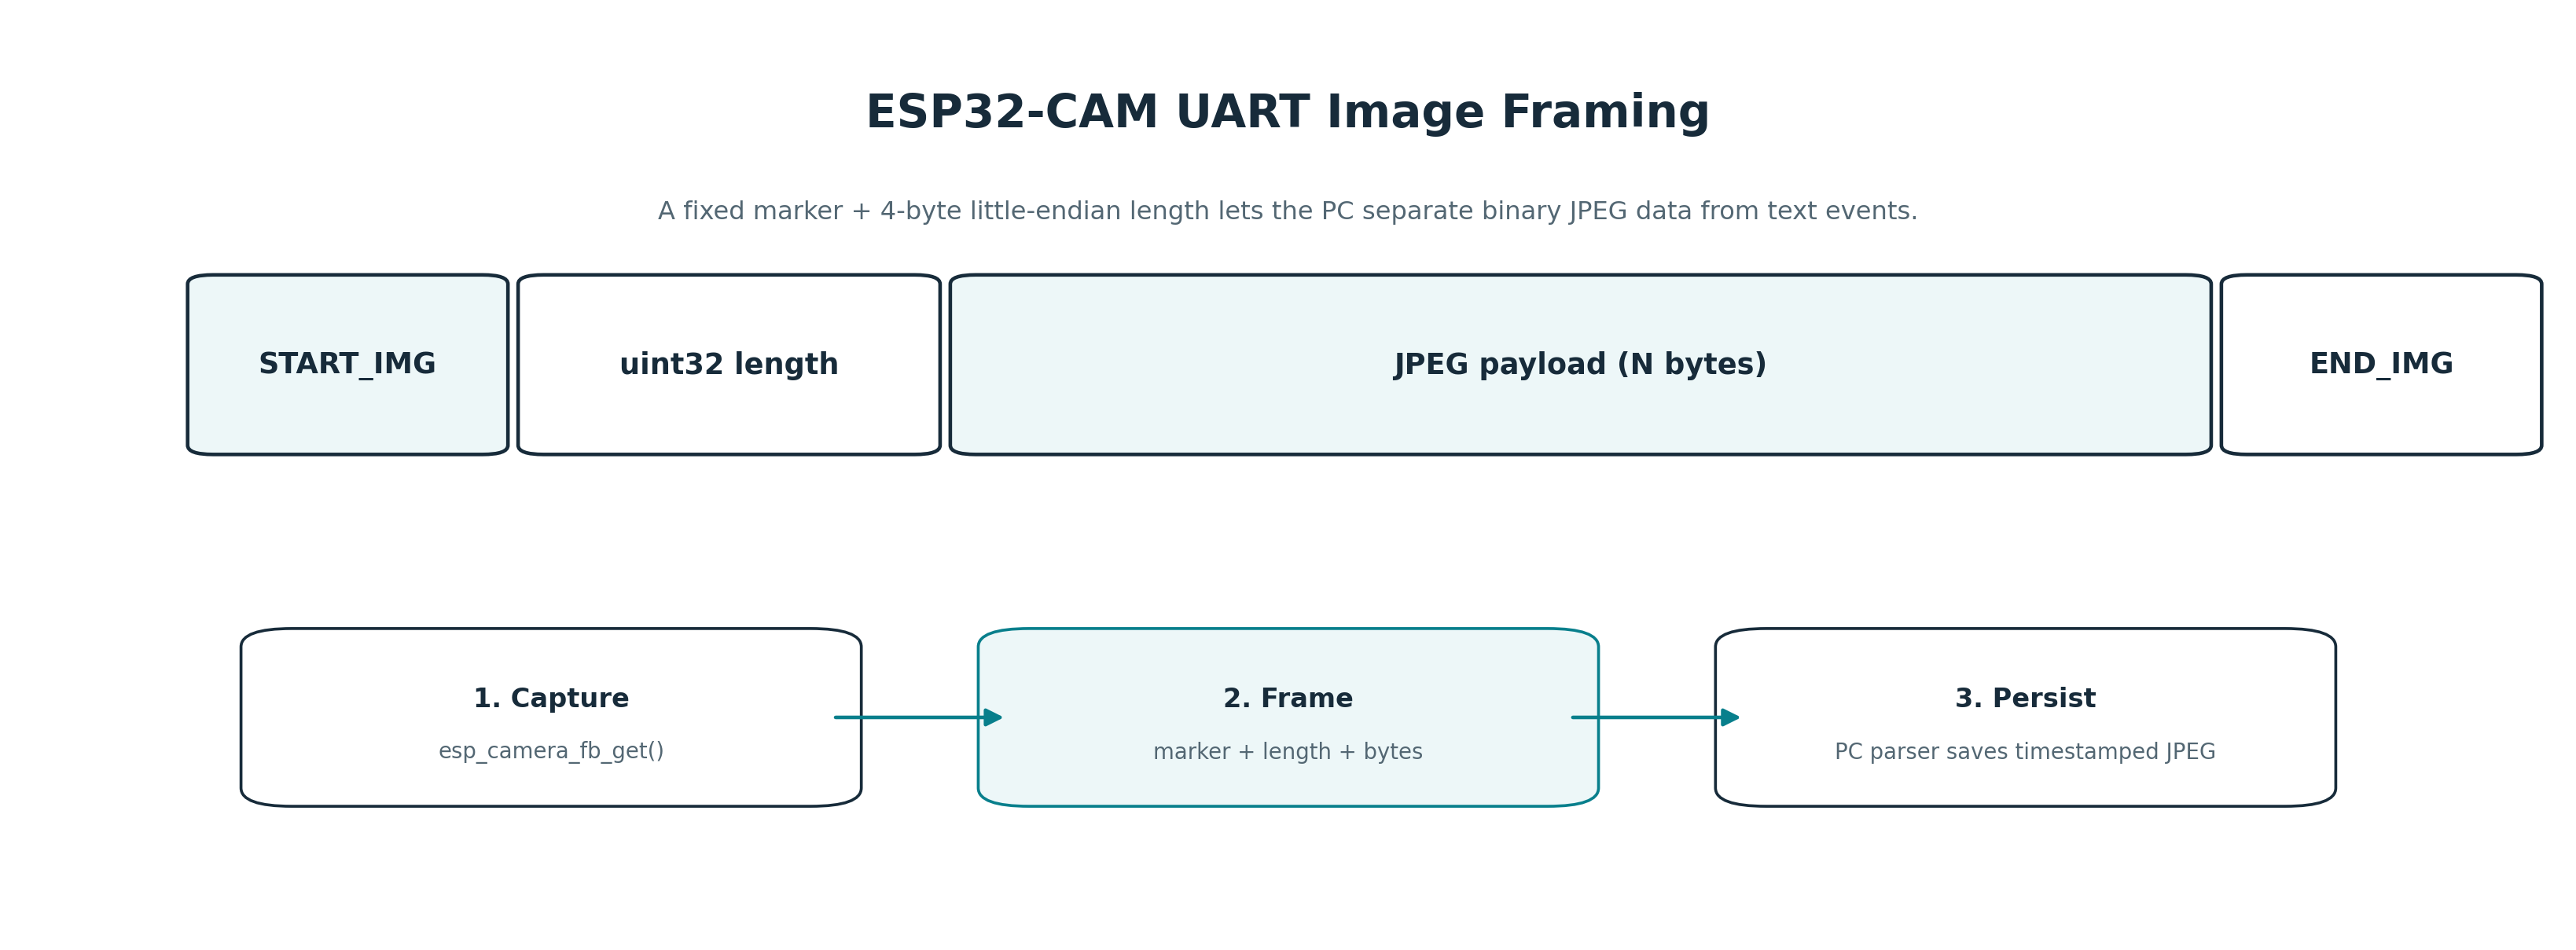
\includegraphics[width=.96\textwidth]{camera_protocol.png}
\caption{قاب انتقال تصویر بین ESP32-CAM و برنامهٔ رایانه}
\label{fig:camera}
\end{figure}

در نسخهٔ اولیه، سمت پایتون چهار بایت برای طول در نظر می‌گیرد و سمت \Eng{ESP32} مقدار \code{size\_t} را با \code{sizeof(length)} می‌فرستد. روی \Eng{ESP32} این مقدار عملاً چهار بایت است، اما قرارداد پروتکل بهتر است وابسته به اندازهٔ نوع دادهٔ کامپایلر نباشد. نسخهٔ آمادهٔ مخزن، طول را صریحاً به \Eng{uint32\_t} تبدیل می‌کند.

\subsection{برآورد زمان انتقال}
در \Eng{UART 8N1} تقریباً برای هر بایت داده ۱۰ بیت روی سیم منتقل می‌شود. بنابراین زمان ایده‌آل انتقال یک تصویر $N$ بایتی در نرخ ۱۱۵۲۰۰ باود تقریباً برابر است با:
\[
T_{UART}(N)\approx \frac{10N}{115200}\;\mathrm{s}.
\]
برای مثال اگر یک فریم ۲۰هزار بایت باشد، فقط زمان انتقال خام حدود $1.74$ ثانیه خواهد بود. این محاسبه توضیح می‌دهد چرا پروژه وضوح \Eng{QVGA} و کیفیت فشرده‌سازی نسبتاً پایین‌تر را انتخاب کرده است.

\subsection{ناهم‌خوانی اسکریپت Tel\_Iot.py}
یک نکتهٔ مهم در تحلیل کد این است که اسکریپت \code{Tel\_Iot.py} پس از ورود، مسیر \code{/capture} را با \Eng{HTTP} فراخوانی و پاسخ را مستقیماً در \code{capture.jpg} ذخیره می‌کند. اما پیاده‌سازی \Eng{ESP32} در این مسیر یک صفحهٔ \Eng{HTML} با پیام «تصویر از UART ارسال شد» برمی‌گرداند؛ خود تصویر هرگز بدنهٔ پاسخ \Eng{HTTP} نیست. بنابراین فایل ذخیره‌شده توسط اسکریپت اولیه، تصویر واقعی نیست. ابزار \code{tools/capture\_request.py} در نسخهٔ مخزن این مشکل را اصلاح می‌کند: مسیر وب را فقط برای \term{فعال‌کردن} تصویربرداری فراخوانی می‌کند و ذخیرهٔ \Eng{JPEG} را به دریافت‌کنندهٔ سریال واگذار می‌کند.

% -----------------------------------------------------------------------------
\section{ماژول تشخیص چهره با DeepFace}
فایل جداگانهٔ \code{Face\_Rec.py} از \code{DeepFace.verify} برای مقایسهٔ یک تصویر پرس‌وجو با دو تصویر مرجع استفاده می‌کند. منطق آن ساده و روشن است: ابتدا مسیرهای \code{1.jpg} و \code{2.jpg} به‌عنوان پایگاه مرجع تعریف شده، \code{3.jpg} به‌عنوان تصویر مقایسه انتخاب می‌شود و حلقه تا نخستین نتیجهٔ \code{verified=True} ادامه می‌یابد. \Eng{DeepFace} یک چارچوب پایتونی برای یکپارچه‌سازی مدل‌ها و عملیات متداول تحلیل چهره است \cite{deepface}.

\begin{notebox}
\textbf{مرزبندی مهم:} در کدهای ارائه‌شده، این اسکریپت به تابع دریافت تصویر از \Eng{ESP32-CAM} متصل نشده است. بنابراین نمی‌توان گفت سامانهٔ اصلی «پس از هر عکس به‌صورت خودکار احراز چهره می‌کند». گزارش فقط می‌تواند نتیجه بگیرد که یک نمونهٔ مستقل برای تطبیق چهره نیز در کنار پروژه وجود داشته است. نسخهٔ گیت‌هاب آن را به ابزار خط فرمانی تبدیل می‌کند که مسیر تصویر پرس‌وجو و پوشهٔ تصاویر مرجع را قابل تنظیم می‌سازد.
\end{notebox}

از منظر امنیت و اخلاق، تصویر چهره دادهٔ زیست‌سنجی حساس است. در مخزن عمومی، پوشهٔ \code{data/reference\_faces} عمداً از گیت حذف می‌شود و استفاده از این ماژول نباید بدون رضایت، حفاظت داده و ارزیابی خطای واقعی به‌عنوان مرز اصلی کنترل دسترسی تلقی شود.

% -----------------------------------------------------------------------------
\section{تحلیل نقاط قوت طراحی}
\begin{itemize}
\item \term{تفکیک زبان طبیعی از فرمان سخت‌افزاری:} تبدیل همهٔ درخواست‌ها به یک الفبای محدود باعث می‌شود بخش سخت‌افزار مستقل از شکل جملهٔ کاربر باشد.
\item \term{چندمسیره‌بودن رابط:} وب محلی، تلگرام و صوت بدون تکرار منطق عملگر به یک مسیر مشترک می‌رسند.
\item \term{تقسیم وظایف بین بردها:} \Eng{ESP32-CAM} وظایف شبکه/دوربین را بر عهده دارد و \Eng{Arduino} عملگرهای ساده را کنترل می‌کند؛ این معماری برای نمایش مفهوم گره‌های ناهمگون در \Eng{IoT} آموزشی است.
\item \term{انتقال صریح تصویر:} استفاده از نشانگر و طول فریم، نسبت به ارسال بایت خام بدون قاب‌بندی قابلیت بازسازی بهتری دارد.
\item \term{بازخورد فیزیکی خطای ورود:} ارتباط رخداد امنیتی وب با بازر روی گرهٔ دیگر نشان‌دهندهٔ یکپارچگی واقعی اجزاست.
\item \term{قابلیت توسعه:} پروتکل حروفی می‌تواند به رله، موتور، حسگر یا گره‌های بیشتر گسترش یابد؛ البته در مقیاس بزرگ بهتر است پیام ساخت‌یافته جایگزین شود.
\end{itemize}

% -----------------------------------------------------------------------------
\section{محدودیت‌ها و اشکالات نسخهٔ اولیه}
بررسی دقیق کد اولیه چند مورد را نشان می‌دهد که در یک پروژهٔ دانشگاهی طبیعی‌اند، ولی برای مخزن عمومی یا توسعهٔ بعدی باید اصلاح شوند.

\subsection{کلیدها و توکن‌های سخت‌کدشده}
در فایل پایتون اولیه، کلید سرویس مدل زبانی و توکن ربات تلگرام مستقیماً داخل کد قرار داده شده‌اند. این مهم‌ترین مشکل انتشار عمومی است. نسخهٔ گیت‌هاب هیچ مقدار واقعی را نگه نمی‌دارد و تنظیمات را از \code{.env} می‌خواند. همچنین اطلاعات شبکه و ورود \Eng{ESP32} به فایل \code{secrets.h} منتقل شده که در \code{.gitignore} قرار دارد.

\begin{warningbox}
اگر کلیدها یا توکن‌های نسخهٔ اولیه قبلاً در هر مخزن، چت اشتراکی یا فایل عمومی قرار گرفته‌اند، فقط حذف آن‌ها از نسخهٔ جدید کافی نیست؛ باید در سرویس مربوطه \term{باطل و مجدداً صادر} شوند.
\end{warningbox}

\subsection{دریافت تصویر دوگانه و مسدودکننده}
در ابتدای \code{IoT.py} تابعی برای انتظار و دریافت تصویر بلافاصله فراخوانی می‌شود؛ این فراخوانی می‌تواند اجرای سایر بخش‌ها را تا زمان رسیدن عکس متوقف کند. پایین‌تر همان فایل، منطق دوم و پیچیده‌تری برای دریافت تصویر در حلقهٔ اصلی وجود دارد. وجود دو مسیر موازی هم احتمال خطا را بالا می‌برد و هم مشخص نیست کدام مسیر منبع حقیقت است. نسخهٔ آمادهٔ مخزن یک \term{parser افزایشی واحد} برای جریان مخلوط متن/باینری دارد.

\subsection{فراخوانی نامعتبر در مسیر باقی‌ماندهٔ داده}
در منطق اولیهٔ دریافت تصویر، عبارتی شبیه \code{self.process\_serial\_data(...)} در یک تابع آزاد وجود دارد؛ در آن محدوده \code{self} تعریف نشده است. همچنین بافر پیش از محاسبهٔ دادهٔ باقی‌مانده پاک می‌شود. این شاخه در بسیاری از اجراها ممکن است فعال نشود، اما از نظر ایستای کد یک خطای روشن است.

\subsection{احراز هویت ساده}
در نسخهٔ اولیه نام کاربری و رمز هر دو مقدار ثابت و بسیار ساده دارند، اطلاعات با \Eng{HTTP} محلی منتقل می‌شود و متغیر \code{isAuthenticated} یک پرچم سراسری برای کل دستگاه است نه نشست مستقل هر مرورگر. این سطح برای دمو قابل درک است، ولی برای محیط واقعی مناسب نیست.

\subsection{وابستگی به سرویس‌های بیرونی}
فرمان تلگرام، تشخیص گفتار و نگاشت مدل زبانی به اتصال اینترنت و سرویس‌های شخص ثالث وابسته است. در صورت قطع اینترنت، مسیر وب محلی همچنان می‌تواند متن را به رایانه برساند، اما اگر تفسیر متن کاملاً به مدل بیرونی وابسته باشد، کنترل طبیعی از کار می‌افتد. یک توسعهٔ مناسب، افزودن parser قطعی محلی برای فرمان‌های رایج است.

% -----------------------------------------------------------------------------
\section{آماده‌سازی نسخهٔ حرفه‌ای برای GitHub}
نسخهٔ همراه گزارش با هدف «انتشارپذیری» و نه بازنویسی ماهیت پروژه تهیه شده است. تغییرات اصلی عبارت‌اند از:
\begin{enumerate}
\item ایجاد ساختار پوشه‌ای روشن شامل \code{src}، \code{firmware}، \code{tools}، \code{docs} و \code{data}؛
\item انتقال تنظیمات حساس و وابسته به سیستم به \code{.env.example} و \code{secrets.h.example}؛
\item افزودن \code{.gitignore} برای جلوگیری از ثبت کلیدها، تصویرها، صوت‌ها و دادهٔ زیست‌سنجی؛
\item بازآرایی برنامهٔ میزبان به کلاس هماهنگ‌کننده و یک parser واحد برای متن و تصویر روی سریال؛
\item اصلاح قرارداد طول تصویر به \Eng{uint32}؛
\item اصلاح اسکریپت درخواست تصویر؛
\item تبدیل اسکریپت \Eng{DeepFace} به ابزار قابل تنظیم بدون مسیر سخت‌کدشدهٔ ویندوز؛
\item مستندسازی کامل روش نصب، فلش‌کردن دو برد، راه‌اندازی و محدودیت‌های امنیتی؛
\item افزودن سه نمودار معماری، جریان فرمان و پروتکل تصویر.
\end{enumerate}

\subsection{ساختار مخزن}
\begin{notebox}
\begin{latin}
\ttfamily\small
IoT-Final-Project/\newline
|-- README.md\newline
|-- SECURITY.md\newline
|-- .env.example\newline
|-- requirements.txt\newline
|-- src/iot\_controller.py\newline
|-- src/face\_verify.py\newline
|-- tools/capture\_request.py\newline
|-- firmware/arduino/Arduino\_IOT.ino\newline
|-- firmware/esp32\_cam/ESP\_AC\_IOT.ino\newline
|-- firmware/esp32\_cam/secrets.h.example\newline
|-- docs/report.tex\newline
`-- docs/figures/...
\end{latin}
\end{notebox}

% -----------------------------------------------------------------------------
\section{راهبرد آزمون و سناریوهای پذیرش}
برای ارزیابی پروژه، آزمون صرفاً «روشن‌شدن یک LED» کافی نیست؛ باید زنجیرهٔ کامل از رابط تا عملگر و نیز مسیر تصویر آزموده شود. جدول زیر مجموعه‌ای از آزمون‌های پذیرش پیشنهادی را ارائه می‌کند.

\begin{table}[H]
\centering
\caption{ماتریس پیشنهادی آزمون سامانه}
\begin{tabularx}{.97\textwidth}{C{1.3cm} R{4.2cm} X}
\toprule
\textbf{ردیف} & \textbf{آزمون} & \textbf{نتیجهٔ مورد انتظار}\\
\midrule
۱ & روشن‌شدن و آماده‌سازی ESP32 & پیام \code{CONFIG\_COMPLETE} در رایانه دریافت شود.\\
۲ & ورود معتبر بدون تلگرام & صفحهٔ پیام باز شود و ربات راه‌اندازی نشود.\\
۳ & ورود معتبر با تلگرام & پیام فعال‌سازی روی سریال دریافت و ربات در رشتهٔ جداگانه شروع شود.\\
۴ & ورود نامعتبر & پیام خطا دریافت و بازر آردوینو حدود نیم ثانیه فعال شود.\\
۵ & فرمان وب برای ESP32 & مدل حرف \Eng{A--F} تولید کند و فقط پورت ESP32 فرمان را دریافت کند.\\
۶ & فرمان وب برای Arduino & مدل حرف \Eng{G--L} تولید کند و فقط پورت Arduino فرمان را دریافت کند.\\
۷ & پیام تلگرام متنی & همان مسیر اعتبارسنجی و مسیریابی فرمان وب طی شود.\\
۸ & پیام تلگرام صوتی & فایل موقت ایجاد، رونویسی، حذف و فرمان اجرا شود.\\
۹ & تصویربرداری & فریم با نشانگر و طول صحیح دریافت و JPEG با نام زمان‌دار ذخیره شود.\\
۱۰ & خروجی نامعتبر مدل & هیچ بایت نامعتبر به هیچ میکروکنترلری ارسال نشود.\\
۱۱ & فرمان E/F & رفتار به‌عنوان رزرو/بدون عمل فیزیکی مستند باشد.\\
۱۲ & تشخیص چهرهٔ مستقل & تصویر پرس‌وجو با مجموعهٔ مرجع مقایسه و نتیجهٔ تطبیق/عدم تطبیق گزارش شود.\\
\bottomrule
\end{tabularx}
\end{table}

\subsection{معیارهای قابل اندازه‌گیری}
برای توسعهٔ بعدی می‌توان زمان انتهابه‌انتها از دریافت پیام تا تغییر خروجی، درصد فرمان‌های مدل که پس از اعتبارسنجی معتبر می‌مانند، نرخ خطای رونویسی صوت، زمان انتقال تصویر و نرخ شکست فریم را ثبت کرد. برای بخش تشخیص چهره نیز ارزیابی واقعی باید با دادهٔ آزمون مستقل و معیارهایی مانند \Eng{FAR/FRR} انجام شود، نه فقط چند تصویر نمونه.

% -----------------------------------------------------------------------------
\section{تحلیل امنیت، حریم خصوصی و قابلیت اطمینان}
\subsection{مدل تهدید پایه}
دارایی‌های مهم سامانه شامل کلیدهای سرویس، توکن تلگرام، اعتبارنامهٔ وب، فرمان‌های سخت‌افزار، تصویر دوربین و تصاویر مرجع چهره هستند. مهاجم بالقوه می‌تواند کاربر غیرمجاز در محدودهٔ \Eng{Wi-Fi}، کاربر تلگرام دارای دسترسی به ربات، یا فردی با دسترسی به مخزن کد باشد.

\subsection{کنترل‌های حداقلی پیشنهادی}
\begin{itemize}
\item چرخش کلیدهای قبلی و نگهداری اسرار خارج از گیت؛
\item رمز قوی برای \Eng{Wi-Fi AP} و حساب وب؛
\item محدودکردن شناسهٔ کاربران/چت‌های مجاز تلگرام؛
\item اعتبارسنجی نهایی هر فرمان پیش از ارسال؛
\item افزودن تأیید دریافت و وضعیت فعلی عملگر برای فرمان‌های مهم؛
\item محدودسازی نرخ درخواست‌های وب و تلگرام؛
\item عدم ثبت تصاویر چهره و تصاویر دوربین در مخزن عمومی؛
\item نگهداری لاگ رخدادها بدون ذخیرهٔ محتوای حساس بیش از نیاز.
\end{itemize}

\subsection{اعتمادپذیری مدل زبانی}
مدل زبانی ممکن است حتی با دستور صریح، خروجی غیرمنتظره تولید کند. به همین دلیل constraint پرامپت به‌تنهایی کنترل امنیتی کافی نیست. کنترل واقعی در سمت برنامهٔ میزبان است: تنها حروف عضو مجموعهٔ مجاز اجازهٔ عبور دارند. در کاربرد حساس‌تر، حتی این روش نیز باید با سیاست مجوز کاربر، ماشین حالت و محدودیت عملیات همراه شود.

% -----------------------------------------------------------------------------
\section{پیشنهادهای توسعهٔ فنی}
\begin{enumerate}
\item \term{پروتکل پیام ساخت‌یافته:} جایگزینی رشته‌ها و تک‌حرف‌ها با فریم دارای نوع پیام، شناسه، طول، \Eng{checksum/CRC} و \Eng{ACK}. برای پروژهٔ بزرگ‌تر، \Eng{MQTT} نیز گزینهٔ طبیعی است.
\item \term{مسیر مستقیم تصویر روی شبکه:} در صورت نیاز به نرخ بالاتر، انتقال \Eng{JPEG} با \Eng{HTTP} یا استریم \Eng{MJPEG} به‌جای \Eng{UART} می‌تواند گلوگاه را کاهش دهد؛ البته این تغییر معماری فعلی را ساده‌تر ولی متفاوت می‌کند.
\item \term{فرمان محلی قطعی:} برای عبارات رایج مانند «چراغ اول را روشن کن» یک parser واژه‌نامه‌ای محلی پیش از مدل زبانی قرار گیرد؛ مدل فقط برای زبان آزاد یا موارد مبهم استفاده شود.
\item \term{ماشین حالت تجهیزات:} وضعیت هر خروجی در نرم‌افزار نگهداری و پاسخ سخت‌افزار تأیید شود تا دستور تکراری یا شکست ارتباط قابل تشخیص باشد.
\item \term{یکپارچه‌سازی اختیاری تشخیص چهره:} پس از دریافت موفق تصویر، یک hook قابل فعال‌سازی می‌تواند \Eng{DeepFace} را اجرا کند؛ بااین‌حال برای کنترل دسترسی واقعی باید تشخیص زنده‌بودن و سیاست حریم خصوصی نیز اضافه شود.
\item \term{آزمون خودکار:} parser سریال را می‌توان بدون سخت‌افزار با تزریق chunkهای مصنوعی آزمود؛ همچنین مسیریاب فرمان با mock پورت سریال قابل تست واحد است.
\item \term{داشبورد وضعیت:} نمایش آخرین فرمان، وضعیت اتصال دو برد، آخرین تصویر و خطاها در یک رابط واحد، قابلیت مشاهده‌پذیری را بالا می‌برد.
\end{enumerate}

% -----------------------------------------------------------------------------
\section{نتیجه‌گیری}
پروژهٔ انجام‌شده یک نمونهٔ نسبتاً کامل از یک سامانهٔ اینترنت اشیای آموزشی است که چند مفهوم مهم را در یک سناریوی واحد کنار هم قرار می‌دهد: شبکهٔ محلی و وب‌سرور روی \Eng{ESP32-CAM}، کنترل عملگر روی دو میکروکنترلر، ارتباط سریال دوطرفه، دریافت و قاب‌بندی تصویر، ربات تلگرام، فرمان صوتی و استفادهٔ محدودشده از مدل زبانی برای تفسیر زبان طبیعی. ارزش اصلی معماری در این است که رابط‌های متنوع در نهایت به یک قرارداد کنترلی کوچک تبدیل می‌شوند و لایهٔ فیزیکی از جزئیات زبان کاربر مستقل باقی می‌ماند.

تحلیل کد نشان داد که نسخهٔ اولیه در سطح نمونهٔ درسی قابل فهم است، اما برای انتشار عمومی باید اسرار از کد خارج شوند، مسیر دریافت تصویر یکپارچه شود، اختلاف اسکریپت \Eng{HTTP} با انتقال واقعی \Eng{UART} اصلاح شود و محدودیت فرمان‌های رزرو مستند گردد. بستهٔ آمادهٔ گیت‌هاب همراه این گزارش این اصلاحات را اعمال می‌کند و در عین حال معماری اصلی پروژه را حفظ می‌کند. اسکریپت \Eng{DeepFace} نیز به‌عنوان ماژول مکمل و مستقل مستندسازی شده است، نه قابلیتی که به‌اشتباه بخشی از مسیر اصلی معرفی شود.

از منظر آموزشی، پروژه نشان می‌دهد که \Eng{IoT} فقط اتصال یک برد به اینترنت نیست؛ مسئلهٔ اصلی طراحی قرارداد بین گره‌ها، کنترل جریان داده، مدیریت ناهمگونی رابط‌ها، تفکیک مسئولیت‌ها و در نظر گرفتن امنیت و قابلیت نگهداری است. با افزودن پروتکل قابل اطمینان‌تر، احراز هویت قوی‌تر، آزمون خودکار و انتقال شبکه‌ای تصویر، همین نمونه می‌تواند مبنای یک سامانهٔ پیشرفته‌تر قرار گیرد.

% -----------------------------------------------------------------------------
\section*{ضمیمه: راهنمای اجرای نسخهٔ مخزن}
\addcontentsline{toc}{section}{ضمیمه: راهنمای اجرای نسخهٔ مخزن}
به‌صورت خلاصه، مراحل اجرای نسخهٔ آمادهٔ گیت‌هاب چنین است:
\begin{enumerate}
\item نصب وابستگی‌ها از \code{requirements.txt}؛
\item کپی \code{.env.example} به \code{.env} و تنظیم پورت‌ها، کلید مدل و توکن تلگرام؛
\item کپی \code{secrets.h.example} به \code{secrets.h} و تنظیم مشخصات شبکه/وب؛
\item فلش \code{firmware/esp32\_cam/ESP\_AC\_IOT.ino} روی \Eng{ESP32-CAM}؛
\item فلش \code{firmware/arduino/Arduino\_IOT.ino} روی \Eng{Arduino}؛
\item اجرای \code{python src/iot\_controller.py}؛
\item اتصال به شبکهٔ ESP32، ورود و آزمایش فرمان‌های وب/تلگرام؛
\item برای تصویربرداری، استفاده از لینک وب یا \code{python tools/capture\_request.py}؛
\item در صورت نیاز به ماژول چهره، نصب \code{requirements-face.txt} و اجرای \code{src/face\_verify.py} روی تصویر ذخیره‌شده.
\end{enumerate}

% -----------------------------------------------------------------------------
{\small
\renewcommand{\refname}{منابع}
\begin{thebibliography}{9}
\setlength{\itemsep}{2pt}
\bibitem{atzori2010}\LRE{Atzori, L., Iera, A., and Morabito, G. (2010). The Internet of Things: A survey. Computer Networks, 54(15), 2787--2805. https://doi.org/10.1016/j.comnet.2010.05.010.}
\bibitem{esp32camera}\LRE{Espressif Systems. esp32-camera: ESP32 compatible camera driver. https://github.com/espressif/esp32-camera.}
\bibitem{ptb}\LRE{python-telegram-bot Documentation. https://docs.python-telegram-bot.org/.}
\bibitem{langchain}\LRE{LangChain Documentation. ChatOpenAI / OpenAI-compatible chat model integration. https://python.langchain.com/docs/integrations/chat/openai/.}
\bibitem{deepface}\LRE{Serengil, S. I., and Ozpinar, A. DeepFace / LightFace face recognition framework and software. https://github.com/serengil/deepface.}
\end{thebibliography}
}

\end{document}
